\documentclass[a4paper, 12pt]{article}
\usepackage[margin=1in]{geometry}
\usepackage{float}
\usepackage{subfigure}
\usepackage[justification=centering]{caption}
\usepackage{enumerate}
\usepackage{multirow}
\usepackage{listings}
\lstset{
    escapechar=`,
    language=C++,
    numbers=left,
    tabsize=2,
    prebreak=\raisebox{0ex}[0ex][0ex]{\ensuremath{\hookleftarrow}},
    frame=single,
    breaklines=true,
}
\usepackage{graphicx}
\graphicspath{ {./} }
\usepackage{nameref}
\usepackage{amsmath}
\usepackage{amssymb}
\usepackage{amsfonts}
\usepackage[linesnumbered,ruled]{algorithm2e}
\usepackage{tikz}
\usetikzlibrary{calc,patterns,decorations.pathmorphing,decorations.markings,positioning,automata}
\usepackage{pgfplots}
\pgfplotsset{compat=1.5}
\usepackage{pgfplotstable}
\usepackage{makecell}
\usepackage{verbatim}
\usepackage[super]{nth}

\begin{document}

% Iterations over DOF
\begin{figure}[H]
  \centering
    \begin{tikzpicture}
      \begin{axis}[
        legend pos=outer north east,
        legend cell align={left},
        grid=both,
        grid style={line width=.1pt, draw=gray!10},
        major grid style={line width=.2pt,draw=gray!50},
        xtick={},
        ytick={},
        ymax=0.11,
        minor tick num=5,
        title=Linear Elastic Beam Bending,
        xlabel=Degrees of Freedom,
        yticklabel style={/pgf/number format/.cd,fixed,fixed zerofill,precision=4,/tikz/.cd},
        ylabel=Iterations ]
        \addplot table {quadratic_data_beam.txt};
          \addlegendentry{Quadratic}
        \addplot table {composite_data_beam.txt};
          \addlegendentry{Composite}
        \addplot table {linear_data_beam.txt};
          \addlegendentry{Linear}
      \end{axis}
    \end{tikzpicture}
  \caption{caption}
  \label{fig:convergence}
\end{figure}

% CPU Time over DOF
\begin{figure}[H]
  \centering
    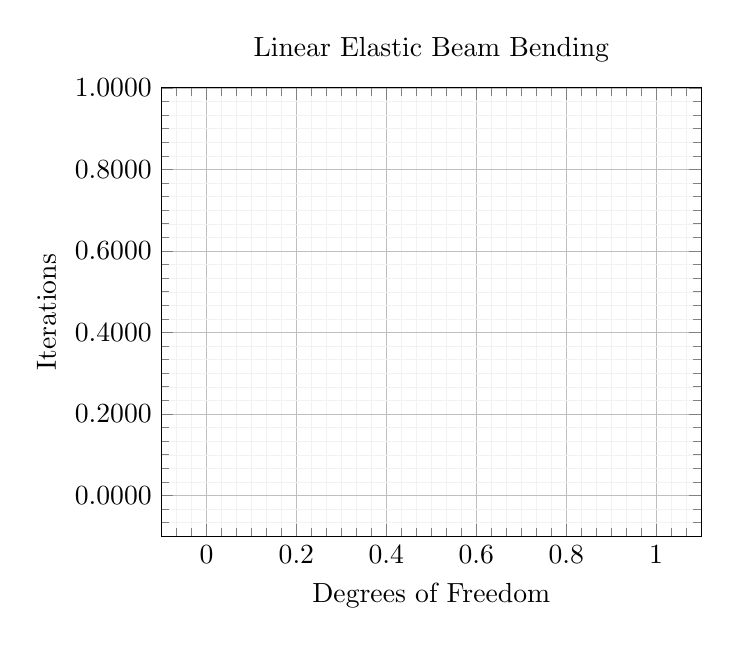
\begin{tikzpicture}
      \begin{axis}[
        legend pos=outer north east,
        legend cell align={left},
        grid=both,
        grid style={line width=.1pt, draw=gray!10},
        major grid style={line width=.2pt,draw=gray!50},
        xtick={},
        ytick={},
        ymax=0.11,
        minor tick num=5,
        title=Linear Elastic Beam Bending,
        xlabel=Degrees of Freedom,
        yticklabel style={/pgf/number format/.cd,fixed,fixed zerofill,precision=4,/tikz/.cd},
        ylabel=Iterations ]
      \end{axis}
    \end{tikzpicture}
  \caption{caption}
  \label{fig:convergence}
\end{figure}


\end{document}
